\documentclass[11pt,a4paper]{article}
\usepackage[utf8]{inputenc}
\usepackage{amsmath}
\usepackage{amsfonts}
\usepackage{amssymb}
\usepackage{multirow,array}
\usepackage[margin=1in]{geometry}
\usepackage{sectsty}
\usepackage[english]{babel}
\usepackage{tikz}
\usepackage{hyperref}

\usetikzlibrary{calc}




\title{Financial Software Engineering exam \\ DOC 5039S}
\author{Luke Meiklejohn
\\MKLLUK001
\\
\\University of Cape Town}

\begin{document}
\maketitle
\pagebreak
\section*{Question 1}
\subsection*{Question 1.1}

To begin we can illustrate the matrix showing the quantities produced by each firm, denoting the two strategies as monopoly (m) and Cuornot (c) with quantities of $\frac{q_m}{2}$ and $q_c$ respectively.
\begin{table}[h]
    \setlength{\extrarowheight}{2pt}
    \begin{center}
    \begin{tabular}{cc|c|c|}
      & \multicolumn{1}{c}{} & \multicolumn{2}{c}{Firm 2}\\
      & \multicolumn{1}{c}{} & \multicolumn{1}{c}{$m$}  & \multicolumn{1}{c}{$c$} \\\cline{3-4}
      \multirow{2}*{Firm 1}  & $m$ & $(\frac{q_m}{2},\frac{q_m}{2})$ & $(\frac{q_m}{2},q_c)$ \\\cline{3-4}
      & $c$ & $(q_c,\frac{q_m}{2})$ & $(q_c,q_c)$ \\\cline{3-4}
	\end{tabular}
	\end{center}
\end{table} 

Each firm has profit function $\pi_i(q_i, q_j) = q_i(a-Q)-cq_i$.
We can solve for the payoffs for each strategy for Firm 1, and get:
$$\pi_1(\frac{q_m}{2}, \frac{q_m}{2}) = \frac{1}{8}(a-c)^2  = 0.125(a-c)^2$$
$$\pi_1(\frac{q_m}{2}, q_c) = \frac{5}{48}(a-c)^2 \approx 0.104(a-c)^2 $$
$$\pi_1(q_c, \frac{q_m}{2}) = \frac{5}{36}(a-c)^2 \approx 0.139(a-c)^2 $$
$$\pi_1(q_c, q_c) = \frac{1}{9}(a-c)^2 \approx 0.111(a-c)^2 $$
This gives the following payoff matrix.
\begin{table}[h]
    \setlength{\extrarowheight}{2pt}
    \begin{center}
    \begin{tabular}{cc|c|c|}
      & \multicolumn{1}{c}{} & \multicolumn{2}{c}{Firm 2}\\
      & \multicolumn{1}{c}{} & \multicolumn{1}{c}{$m$}  & \multicolumn{1}{c}{$c$} \\\cline{3-4}
      \multirow{2}*{Firm 1}  & $m$ & $(0.125(a-c)^2,0.125(a-c)^2)$ & $(0.104(a-c)^2,0.139(a-c)^2)$ \\\cline{3-4}
      & $c$ & $(0.139(a-c)^2,0.104(a-c)^2)$ & $(0.111(a-c)^2,0.111(a-c)^2)$ \\\cline{3-4}
	\end{tabular}
	\end{center}
\end{table}

Noting that $\frac{q_m}{2} < q_c$, we can see that if Firm 2 chooses strategy m (to produce $\frac{q_m}{2}$), Firm 1 has an incentive to deviate and choose strategy c, producing $q_c$. Similarly, if Firm 2 chooses strategy c, Firm 1 has an incentive to produce strategy c again. It is clear that for Firm 1, strategy m is \textit{strictly dominated} by strategy c - given Firm 2's choices, Firm 1 never has an incentive to choose strategy m to produce $\frac{q_m}{2}$.

The same is true for Firm 2 given Firm 1's choices - strategy m is \textit{strictly dominated} by strategy c.

The equilibrium quantities are found as follows. Suppose Firm 1 chooses strategy m. Then it is in Firm 2's incentive to produce the higher quantity $q_c$ with strategy c. However, given that Firm 2 chooses strategy c, it is in Firm 1's interest to produce quantity $q_c$ also.

Each firm's profit is calculated as: $$\pi_i (q_c, q_c) = q_i \times P(Q) - c\times q_i $$
$$ \pi_i (q_c, q_c) = q_i(a-Q)-cq_i = \frac{a-c}{3}(a-\frac{2(a-c)}{3})-c\frac{a-c}{3}$$
$$ = \frac{a-c}{3}\Big(a-\frac{2(a-c)}{3}-c\Big) = \frac{a-c}{3}\Big(\frac{3a-2a+2c-3c}{3}\Big) = \frac{a-c}{3}\Big(\frac{a-c}{3}\Big)$$
$$ \Rightarrow \pi_i (q_c, q_c) = \frac{(a-c)^2}{9}$$

If we consider the case where both firms choose the monopoly strategy, each firm's profit is:
$$\pi_i (q_m, q_m) = q_i \times P(Q) - c\times q_i $$
$$ \pi_i (q_c, q_c) = q_i(a-Q)-cq_i = \frac{a-c}{4}(a-\frac{2(a-c)}{4})-c\frac{a-c}{4}$$
$$ = \frac{a-c}{4}\Big(a-\frac{a-c}{2}-c\Big) = \frac{a-c}{4}\Big(\frac{2a-a+c-2c}{2}\Big) = \frac{a-c}{4}\Big(\frac{a-c}{2}\Big)$$
$$ \Rightarrow \pi_i (q_m, q_m) = \frac{(a-c)^2}{8} > \pi_i (q_m, q_m)$$

So, through not coordinating, both firms are worse off and make a smaller profit. 

To answer the second part to the question, we consider that before, strategy m was strictly dominated by strategy c. For there to no longer be any strict domination, we must have that the quantity $q'$ is the best response for one of the strategies, or allows strategy m to be the best response (1). We also know that $(q_c, q_c)$ is the equilibrium quantity produced, so this means that $(q',q')$ cannot be an equilibrium.
The matrix showing the possible quantities produced is below, calling the third strategy (*).

\begin{table}[h]
\setlength{\extrarowheight}{2pt}
\begin{center}
\begin{tabular}{cc|c|c|c|}
  & \multicolumn{1}{c}{} & \multicolumn{3}{c}{Firm $2$} \\
  & \multicolumn{1}{c}{} & \multicolumn{1}{c}{$m$}  & \multicolumn{1}{c}{$c$}  & \multicolumn{1}{c}{$(*)$} \\\cline{3-5}
            & $m$ & $(\frac{q_m}{2},\frac{q_m}{2})$ & $(\frac{q_m}{2},q_c)$ & $(\frac{q_m}{2},q')$ \\ \cline{3-5}
Firm $1$    & $c$ & $(q_c,\frac{q_m}{2})$ & $(q_c,q_c)$ & $(q_c,q')$ \\\cline{3-5}
            & $(*)$ & $(q',\frac{q_m}{2})$ & $(q',q_c)$ & $(q',q')$ \\\cline{3-5}
\end{tabular}
\end{center}
\end{table}

Given that Firm 1 chooses to produce $q'$, Firm 2 must thus choose either strategy m or c - so, the profit made from one of these strategies must be higher than the profit earned through producing $q'$. 

If we suppose from (1) that $\frac{q_m}{2}$ is the best response to $q'$, then we can calculate, from the best response function for Firm 1, $R(q_2) = \frac{1}{2}(a-c-q') \Rightarrow \frac{q_m}{2} = \frac{1}{2}(a-c-q') $
$$\Rightarrow q' = a-c-q_m = a-c-\frac{a-c}{4} = \frac{4a-4c-a+c}{4} = \frac{3}{4}(a-c)$$

\subsection*{Question 1.2}

Firms 2 and 3 will choose their optimal quantities as in the Cuornot model, since Firm 1's choice will already have taken place. They will this seek to maximise their profit functions as follows - lets take Firm 3.
$$ \max_{q_3} \Big( q_3 \times P(Q) - cq_3 \Big) = \max_{q_3}\Big( q_3(a-q_1^*-q_2-q_3)\Big)$$
Which is equivalent to solving:
$$ \Rightarrow \frac{\partial \pi_3}{\partial q_3} = a-q_1-q_2-2q_3-c = 0$$
$$ \Rightarrow q_3 = \frac{a-q_1-q_2-c}{2}$$
Similarly, $q_2 = \frac{a-q_1-q_3-c}{2}$.

We can solve for $q_1$ and $q_2$ by first noting that they will produce the same quantities since they face the same information, and so $q_1 = q_2$.

$$ \Rightarrow q_2 + \frac{1}{2}q_2 = \frac{a-q_1-c}{2} \Rightarrow q_2^* = q_3^* = \frac{a-q_1-c}{3}$$

We can now proceed to solve for Firm 1's quantity chosen, given that they know what Firm 2 and 3's responses will be. This is equivalent to solving 
$$\max_{q_1}\pi_1(q_1,q_2^*,q_3^*) = \max_{q_1} \; q_1(a-q_1-q_2^* - q_3^*) - cq_1 = \max_{q_1} q_1\Big(a-q_1-\frac{2(a-q_1-c)}{3}\Big) - cq_1 $$
$$ = \max_{q_1}\; q_1\frac{3a-3q_1-2a+2q_1+2q_1+2c-3c}{3} = \max_{q_1}\; q_1 \Big(\frac{a-q_1-c}{3}\Big)$$
Similarly to before, we equate the partial derivative to zero to maximise it.
$$ \frac{\partial \pi_1}{\partial q_1} = \frac{a-2q_1-c}{3} = 0 \Rightarrow q_1^* = \frac{a-c}{2}$$

\subsection*{Question 1.3}

A repeated game is played over discrete time periods  $\{1, 2, ..., N\}$, whereby each player plays an action $A_i$ at time point $i$.

In a repeated game, a \textit{strategy} is a sequence of the actions taken by a player in each round. That is, a strategy is of the form $\{A_1^*, A_2^*, ..., A_N^*\}$.

A \textit{subgame} is the static game that is played at time point $i$ - it starts at a decision node with one piece of information showing the strategies that have been played already, and it includes all possible decisions or outcomes that could follow that node.

A \textit{subgame perfect Nash equilibrium} is a final outcome which represents a Nash equilibrium in every subgame of the game. That is, every subgame equilibria are Nash equilibria: in each subgame, the decisions played by each player are the ones which give the best outcome.

\subsection*{Question 1.4}

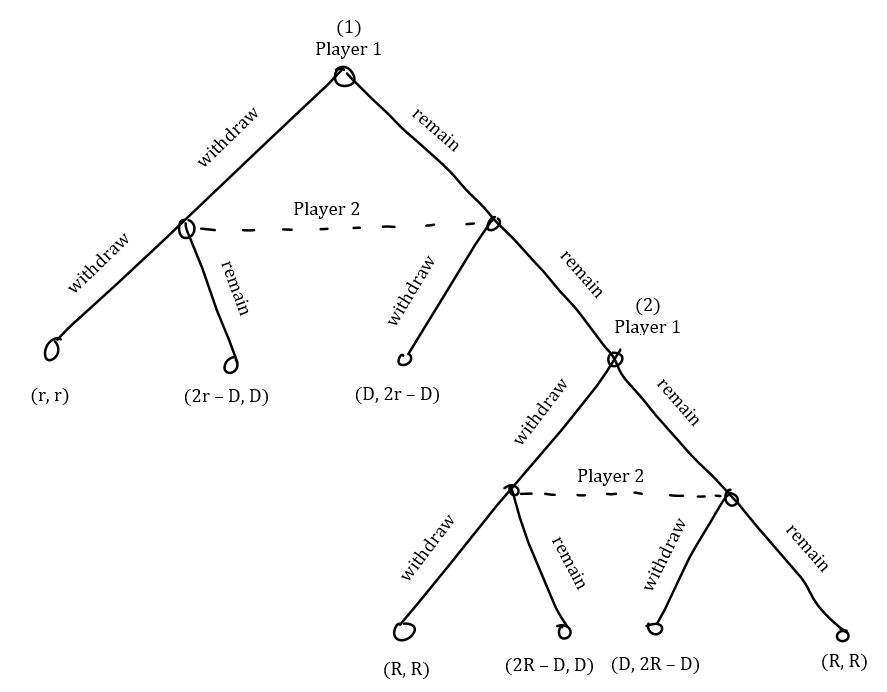
\includegraphics[width=\textwidth]{Fig.JPG} 



The extensive form can be represented in the above graph. It includes:
\begin{itemize}
\item The order of moves: in the graph it is represented as Player 1 moving and then Player 2 moving, but the dotted lines indicate that Player 2 has an incomplete information set - they do not know Player 1's move, so the form is correct in representing that Player 1 and Player 2 move at the same time. They both either choose to Withdraw or Remain at step 1, and then the same choice at step 2. 
\item The actions taken at each stage of the game - either Withdraw or Remain
\item The information available during the game - only at the outcome nodes do the players know the move of the other player. The exception is at decision node 2, where each player knows the moves played in the previous step.
\end{itemize}
The strategic form consists of:
\begin{itemize}
\item The set of players $\{P_1, P_2\}$
\item For each player $P_i$, a set of actions. For Player 2 this is the following: 

If Player 1 chooses to Withdraw at step 1,  \{\{Remain\}, \{Withdraw\}\}

If Player 1 chooses to Remain at step 1, \{\{Remain, Remain\}, \{Remain, Withdraw\}\}

The payoffs for the second set are dependent on Player 1's action at step 2.

\item The payoffs for each possible strategy - again we will illustrate them for Player 2. 

If Player 1 chooses to Withdraw at step 1 the payoffs are $\{(r,r), (2r-D)\}$

If Player 1 chooses to Remain at step 1:

And chooses to Withdraw at step 2: $\{(2R-D, D),(R, R)\}$

And chooses to Remain at step 2: $\{(R, R),(2R-D, D)\}$
\end{itemize}

Noting that to Withdraw dominates to Remain at step 2, the payoffs in a one-shot game are illustrated in this payoff matrix.

\begin{table}[h]
    \setlength{\extrarowheight}{2pt}
    \begin{center}
    \begin{tabular}{cc|c|c|}
      & \multicolumn{1}{c}{} & \multicolumn{2}{c}{Player 2}\\
      & \multicolumn{1}{c}{} & \multicolumn{1}{c}{$withdraw$}  & \multicolumn{1}{c}{$remain$} \\\cline{3-4}
      \multirow{2}*{Player 1}  & $withdraw$ & $(r,r)$ & $(D,2r-D)$ \\\cline{3-4}
      & $remain$ & $(2r-D,D)$ & $(R, R)$ \\\cline{3-4}
	\end{tabular}
	\end{center}
\end{table} 

The two pure-strategy subgame-perfect equilibria are for both parties to Remain at step 1 and then Withdraw at step 2, and to both Withdraw at step 1.

\subsection*{Question 1.5}

Firm $i$'s action space is the set of all prices they can sell at, that is $A_i = \{p: p \geq 0\}$.
Firm $i$'s type space is the set of all sensitivities that they can have, that is $T_i = \{b_{iH}, b_{iL}\}$ with $\Pr(b_{iH}) = h$ and $\Pr(b_{iL}) = 1-h$. (I have changed the notation slightly to be clear that $b_{iH}$ is the sensitivity of Firm $i$).

Firm $i$ only knows $b_i$, not $b_j$.

Firm $i$ has utility function $$u_i(b_i,p_i,p_j) = \begin{cases} 
      (a-p_i-b_ip_j)p_i & \text{if} \; p_i \leq a-bp_j \\
      0 & \text{otherwise} \\
\end{cases} $$
   
Firm $i$'s strategy space is the set of all possible strategies, that is $\{(p_{iH},p_{iL}): p_{iH}, p_{iL} \in A_i \}$.

The symmetric pure-strategy Bayesian Nash equilibrium is one where Firm $i$ and $j$ both produce at the same price, that is, when $$b_i = b_j = b_L \Rightarrow p_i = p_j$$ and when $$b_i = b_j = b_H \Rightarrow p_i = p_j$$

Each firm will solve $$\max_{p_i} \Big\{ h (a - p_i - b_i p_{j}^{L}) p_i + (1-h) (a - p_i - b_i p_{j}^{H}) p_i \Big\}$$

Which we do through equating the partial derivative to zero as before.

%$$h(a-p_i-b_ip_j^L)-2hp_i+(1-h)(a-p_i-b_ip_j^H)-2(1-h)p_i = 0 $$

Let $f(p_i) = hp_i(a-b_ip_j^L)-hp_i^2 + (1-h)p_i(a-p_j^H)-(1-h)p_i^2 $

Then

$$\frac{\partial f}{\partial p_i} = h(a-b_ip_j^L) - 2hp_i + (1-h)(a-p_j^H) - 2(1-h)p_i $$
$$ \Rightarrow p_i(-2h-2+2h) = -h(a-b_ip_j^L) + (1-h)(a-b_ip_j^H) $$
$$ \Rightarrow p_i = \frac{h(a-b_ip_j^L)+(1-h)(a-b_ip_j^H)}{2}$$

We are finding the symmetric equilibrium hence we must have $p_i^L = p_j^L = p_L^*$ and $p_i^H = p_j^H = p_H^*$, so we can solve for these:

$$p_L^* = \frac{h(a-b_L p_L^*)+(1-h)(a-b_Lp_H^*)}{2}$$
$$2p_L^* + hb_Lp_L^* = ha+(1-h)(a-b_Lp_H^*)$$
$$p_L^*(2+hb_L) = a-(1-h)b_Lp_H^*$$
$$ \Rightarrow p_L^* = \frac{a-(1-h)b_Lp_H^*}{2+hb_L} $$

Similarly, for $p_H^*$:

$$p_H^* = \frac{h(a-b_Hp_L^*)+(1-h)(a-b_hp_H^*)}{2} $$
$$ 2p_H^* +b_Hp_H^* - b_Hp_H^* = ha-hb_Hp_L^*-ha+a$$
$$ p_H^*(2+b_H-hb_H) = a - hb_Hp_L^* $$
$$ \Rightarrow p_H^* = \frac{a-hb_Hp_L^*}{2+(1-h)b_H} $$

Using WolframAlpha to solve these equations simultaneously (see \href{https://bit.ly/2TFDSfE}{here}) gives:

$$p_H^* = \frac{a}{2}\Big( \frac{h(b_L-b_H)+2}{-hb_H+hb_L+b_H+2} \Big) = \frac{a}{2} \Big( \frac{h(b_L-b_H)+2}{hb_L+(1-h)b_H+2} \Big)$$
$$p_L^* = \frac{a}{2}\Big( \frac{b_H(h-1)-hb_L+b_L-2}{(h-1)b_H-(hb_L+2)} \Big) = \frac{a}{2}\Big( \frac{(1-h)(b_H-b_L)+2}{(1-h)b_H +hb_L + 2} \Big)$$

For this to be a valid equilibrium, the following condition must be met:

$$p_L^*, p_H^*, q(p_H^*, p_H^*), q(p_H^*,p_L^*), q(p_L^*, q_H^*), q(p_L^*, p_L^*) > 0$$

That is, all of the possible prices and quantities must be positive. 

\subsection*{Question 1.6}

There are $n$ bidders, each with private valuations $v_i$.

They each place bids $b_i$.

Their payoffs, after the auction has been realised, are:

$$u_i(b_i,b_{-i}, v_i) =  \begin{cases} 
      v_i-b_i & b_i>b_i \; \forall j \neq i 0 \\
      0 & \text{otherwise} \\
   \end{cases}
$$

What we will show is that $(s_1^*, s_2^*, ..., s_n^*)$ is a symmetric Bayesian Nash Equilibrium, where $s_i^*(b_i) = \frac{n-1}{n}b_i$. So, we show that this strategy solves:

\begin{align*}
\max_{b_i} (v_i-b_i) \Pr[b_i \geq b_j, \forall j \neq i] \\
= \max_{b_i} \;(v_i-b_i) \Pr\Big[b_i \geq \frac{n-1}{n}v_j, \forall j \neq i\Big] \\
= \max_{b_i} \;(v_i-b_i) \prod_{j \neq i} \Pr\Big[b_i \geq \frac{n-1}{n} v_j\Big] && \text{from independence}\\
= \max_{b_i} \;(v_i-b_i) \prod_{j \neq i} \Pr\Big[v_j \leq \frac{n}{n-1}b_i\Big] \\
= \max_{b_i} \;(v_i-b_i) \prod_{j \neq i} \Big(\frac{n}{n-1}b_i\Big) && \text{from uniformity}  \\
= \max_{b_i} \;(v_i-b_i) \Big(\frac{n}{n-1}b_i\Big)^{n-1} && (2) \; \text{from identicality}  \\
\end{align*}
Solving the above is equivalent to equating the partial derivative with respect to $b_i$ to zero and solving for $b_i$.
The partial derivative is:
\begin{align*}
(n-1)\Big(\frac{n}{n-1}\Big)^{n-1}v_i b_i^{n-2} - n\Big(\frac{n}{n-1}\Big)^{n-1}b_i^{n-1} && (3)
\end{align*}
Rather than solve for $b_i$, we substitute in $\hat{b}_i = \frac{n-1}{n}v_i$ and check that this is a local maximum of (2).
\begin{align*}
(n-1)\Big(\frac{n}{n-1}\Big)^{n-1}v_i\Big(\frac{n-1}{n}\Big)^{n-2}v_i^{n-2} - n\Big(\frac{n}{n-1}\Big)^{n-1}\Big(\frac{n-1}{n}\Big)^{n-1}v_i^{n-1} \\
= nv_i^{n-1} - nv_i^{n-1} \\
= 0 
\end{align*}

Therefore the strategy $b_i = \frac{n-1}{n}v_i$ maximises (2).

Hence the strategy is symmetric and a unique Bayesian Nash Equilibrium.

\subsection*{Question 1.7}

We proceed in much the same fashion as for \textbf{1.6}.

The payoffs for each bidder, after the auction has been realised, are:

$$u_i(b_i,b_{-i}, v_i) =  \begin{cases} 
      v_i-b_i & b_i>b_i \; \forall j \neq i 0 \\
      0 & \text{otherwise} \\
   \end{cases}
$$

So each bidder faces the following maximisation problem:
\begin{align*}
 \max_{b_i} \;(v_i-b_i) \Pr[b_i > b_j \; \forall j \neq i] \\
 = \max_{b_i}\; (v_i-b_i) \prod_{j \neq i} \Pr[b_i > b_j]
\end{align*}

Each bidder will choose a strategy $s_i(v_i) = b_i$.

We seek to find the symmetric Bayesian Nash equilibrium $(s_1^*, s_2^*, ..., s_n^*)$.

We consider the case where $s_i(v_i) = b_i = \alpha v_i$, that is each bidder bids some linear multiple of their private valuation ($\alpha > 0$). Then we have:

\begin{align*}
\max_{b_i}\; (v_i-b_i) \prod_{j \neq i} \Pr[b_i>\alpha v_i] = \max_{b_i} (v_i-b_i) \prod_{j \neq i} \Pr[v_i < \frac{1}{\alpha}b_i]
\end{align*}

Since we are dealing with the simplified case of there being only two bidders, we solve the following for Player 1:

\begin{align*}
\max_{b_1} \; (v_1-b_1) \Pr[v_2 < \frac{1}{\alpha} b_1] && \text{(4)}
\end{align*}

We know that valuations are independently and identically distributed according to some probability distribution function $f$, so we denote the \textit{cumulative} distribution function by $F$. Then we can express (4) as:

\begin{align*}
\max_{b_1}\; (v_1-b_1) F(\frac{1}{\alpha}b_1) 
\end{align*}

We let $g(b_1) = (v_1-b_1)F(\frac{1}{\alpha}b_1)$ and maximise the above by taking the derivative with respect to $b_1$.

\begin{align*}
\frac{\partial g}{\partial b_1} = v_1 f(\frac{1}{\alpha}b_1)\frac{1}{\alpha} - F(\frac{1}{\alpha}b_1) - b_1 f(\frac{1}{\alpha}b_1)\frac{1}{\alpha}
\end{align*}

At the maximum of $g$, the above will be equal to $0$. So we consider the case of $\hat{b}_1 = \frac{1}{2}v_1$ and show that this indeed maximises $g$.

\begin{align*}
\frac{\partial g}{\partial b_1} = v_1 f(2\frac{1}{2}v_1)2-F(v_1)-\frac{1}{2}v_1f(v_1)2 = 2v_1f(v_1)-F(v_1)-v_1f(v_1) \\
= v_1f(v_1)-F(v_1) \\
= -F(v_1) + F'(v_1)(v_1 - 0) \\
= -F(v_1) - F'(v_1)(0-v_1)
\end{align*}

Now, we recognize that the first-order Taylor expansion of $F(x)$ about $v_1$ is: $$F(x) \approx F(v_1)+F'(v_1)(x-v_1)$$

Hence we can say that $F(0) \approx F(v_1)+F'(v_1)(0-v_1)$. So:
\begin{align*}
\frac{\partial g}{\partial b_1} \approx -F(0) = 0
\end{align*}

This proves that $\alpha = \frac{1}{2}$ maximises the payoffs for the two bidders and the symmetric Bayesian Nash Equilibrium is thus again $$(s_1^*(v_1),s_2^*(v_2))=(\frac{n-1}{n}v_1, \frac{n-1}{n}v_2) = (\frac{1}{2}v_1,\frac{1}{2}v_2)$$

\end{document}